\documentclass[12pt]{exam}

\usepackage{ge05}
\usepackage{comment}
\usepackage{booktabs}
\usepackage[dvipdfm]{hyperref}
\urlstyle{rm}   % change fonts for url's (from Chad Jones)
\hypersetup{
    colorlinks=true,        % kills boxes
    allcolors=blue,
    pdfsubject={NYU Stern course GB 2303, Global Economy},
    pdfauthor={Dave Backus @ NYU},
    pdfstartview={FitH},
    pdfpagemode={UseNone},
%    pdfnewwindow=true,      % links in new window
%    linkcolor=blue,         % color of internal links
%    citecolor=blue,         % color of links to bibliography
%    filecolor=blue,         % color of file links
%    urlcolor=blue           % color of external links
% see:  http://www.tug.org/applications/hyperref/manual.html
}

% for ge05.sty
\def\ClassName{The Global Economy}
%\def\Category{Professor David Backus}
\def\Category{Backus \& Cooley}
\def\HeadName{Problem Set \#3}
\newcommand{\phm}{\phantom{--}}
\newcommand{\NX}{\mbox{\it NX\/}}
\newcommand{\POP}{\mbox{\it POP\/}}

\printanswers

\begin{document}
\parindent = 0.0in
\parskip = \bigskipamount
\thispagestyle{empty}%
\Head

\centerline{\large \bf \HeadName: Macroeconomic Indicators}
\centerline{Revised:  \today}

\medskip
{\it You may do this assignment in a group of up to five people.
Whatever you hand in should be the work of your group.}

\begin{questions}
% --------------------------------------------------------------------
\question Cyclical businesses (20 points).
Rate each of the following businesses
as not cyclical, cyclical, or very cyclical.
Explain your reasoning.
\begin{parts}
\part Machine tools (5~points)
\part Grocery stores (5~points)
\part Family practice medicine (5~points)
\part Mercedes S-class sedans (5~points)
\end{parts}

\begin{solution}
\begin{parts}
\part Durable good, very cyclical.
\part Nondurable good, slightly cyclical.
\part Service, not cyclical (or not very cyclical).
\part Luxury good, very cyclical.
\end{parts}
\end{solution}

\question Monthly indicators (40 points).
The idea is to review some of the tools we've developed
to establish cyclical patterns of various
economic indicators.

We'll use data from the St Louis Fed's
\href{http://research.stlouisfed.org/fred2/}{FRED}.
Download monthly data from 1990 to the present
for industrial production (series INDPRO),
nonfarm employment (PAYEMS),
housing starts (HOUST),
retail sales (RRSFS, starts in 1992),
and the S\&P 500 stock market index (SP500).

Construct year-on-year growth rates for each series.
With them in hand:
\begin{parts}
\part
Compute and report the standard deviation of each one.
(10~points)

\part
Compute and report the correlation of each variable with industrial production.
Which variable has the highest correlation?
Are any of them countercyclical?
(10~points)

\part Compute cross-correlation functions for each variable with industrial
production.
Which variables are leading indicators?
Which are lagging indicators?
(20~points)
\end{parts}

\begin{solution}
\begin{parts}
\part See below.  These numbers are for growth rates computed in FRED,
what they call ``percent change from a year ago.''
If you use continuously-compounded growth rates, the numbers will be a little different.

\begin{center}
\begin{tabular}{lrrr}
\toprule
Series                  &  mean & std dev  & corr w/ IP \\
\midrule
Industrial production   & 2.03  &  4.34    &  1.00   \\
Nonfarm employment      & 0.91  &  1.78     & 0.81 \\
Housing starts          & --1.68& 17.67    &  0.52 \\
Retail sales            &2.06   &  3.53    &  0.80  \\
S\&P 500 index          & 7.92  & 17.19    &  0.65  \\
\bottomrule
\end{tabular}
\end{center}

\part See last column above.
All the correlations are positive in this case.
The largest one with with employment, with retail
sales a close second.

\part Cross-correlation functions below.
The ones we used in class start in 1960, these start in 1990.

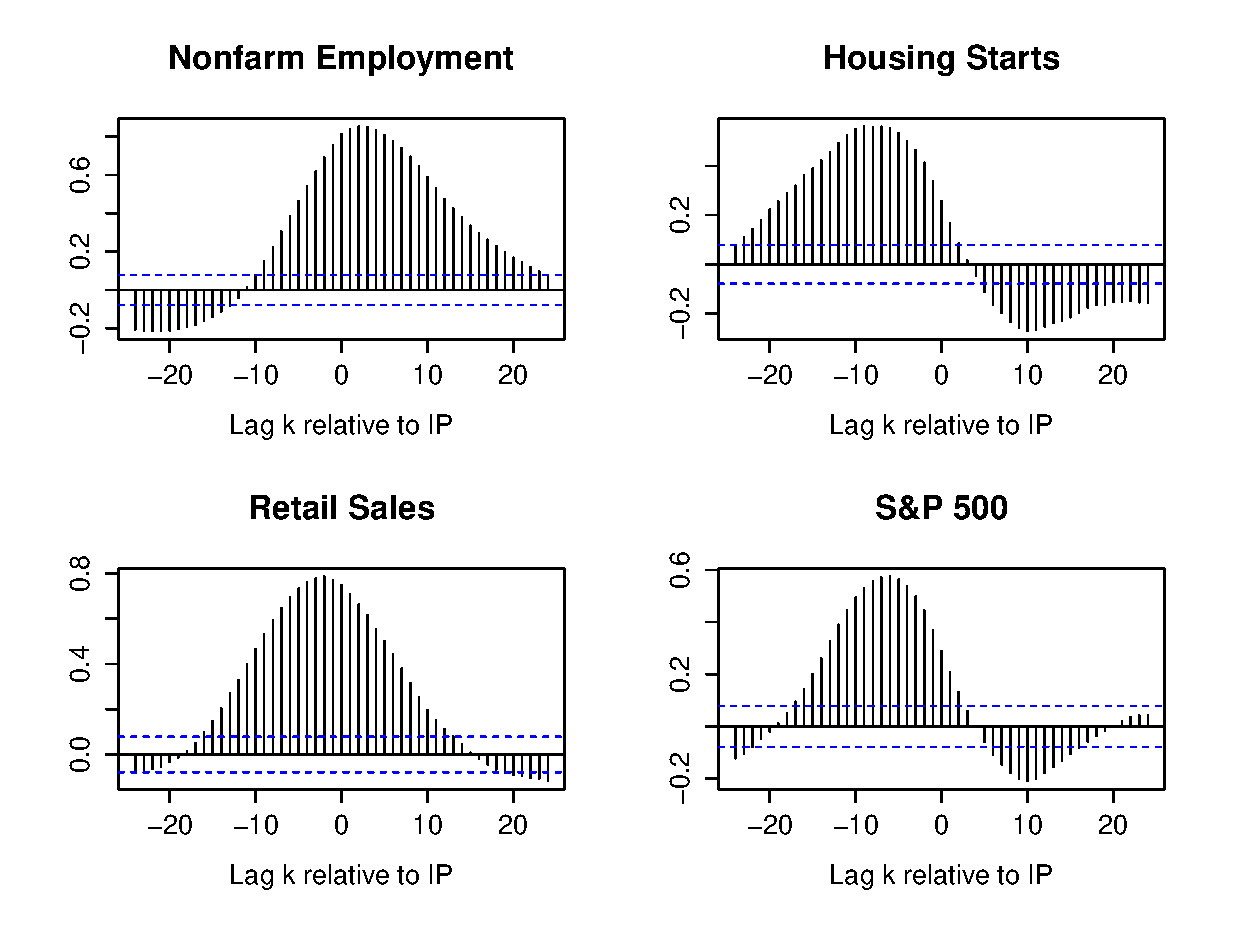
\includegraphics[width=0.85\textwidth]{ps3_q2_ccfs.eps}

PS:  These were computed in R,
a popular open-source statistics program.
If you think you'd like to try it, let me know and I'll send you
the program.

\end{parts}
\end{solution}

% --------------------------------------------------------------------
\question Near-term economic conditions (40 points)
You are delighted to have a summer internship in JP Morgan's
capital markets group.
Your first rotation:  Fixed Income Research.
On your first day, the Managing Director gives you
a small project to get your feet wet.
Noting that bond markets are driven largely by macroeconomic news,
she asks you to write a report summarizing the near-term prospects for the US
economy, specifically the next two quarters.

You go (again) to FRED or other source
and download 8-10 of your favorite economic indicators.
(If you're short of ideas, look at the Bloomberg
\href{http://www.bloomberg.com/markets/economic-calendar/}{economic calendar}
and the macroeconomic
\href{http://pages.stern.nyu.edu/~dbackus/macro_resources.htm}{resource page}.)
After transforming them as needed,
you:
%
\begin{parts}
\part Explain (briefly) why you chose each of your indicators,
and whether you think it's better to use the indicator,
its growth rate, or some other ``transformation.''
(10~points)

\part Graph each indicator (suitably transformed) over some sensible sample period.
What are the advantages of a long sample period?  Disadvantages?
Include on the graph lines representing
the sample mean and plus/minus one standard deviation.
(10~points)

\part Summarize your findings in a business cycle scorecard,
as outlined in the notes.
(10~points)

\part Overall, do they indicate above-average, below-average,
or average growth of the US economy?
What judgemental factors would you add to your analysis?
Where do you think the US economy is headed?
(10~points)
\end{parts}

\begin{solution}
You'll have to use your own judgement here.
Part of the judgement involves which series to use.
Generally you want to use series whose ups and downs
are highly correlated with those of the economy.  
Another part is whether to use levels or growth rates.
Generally you want to use whatever works best, 
but there's no mechanical method to determine that. 
With housing starts, for example, the growth rate looks pretty good, 
but the level still looks bad.  
Which is it?  Hard to say, we haven't been in this situation before.   

The plot below includes four of the series (their growth rates) 
we looked at above
with the requested lines added.

\begin{center}
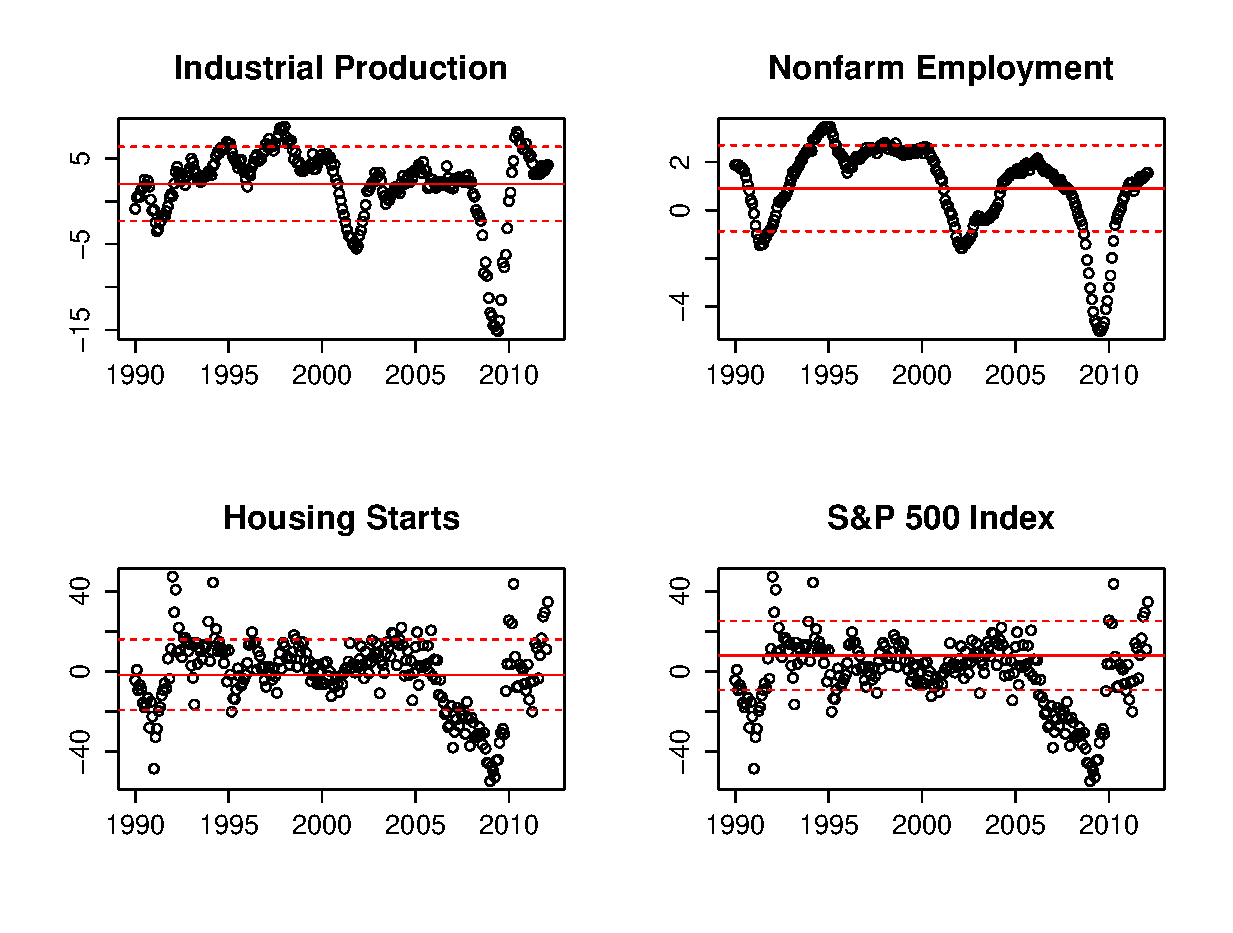
\includegraphics[width=0.85\textwidth]{ps3_q3_scorecard.eps}
\end{center}

\end{solution}

\end{questions}

\vfill \centerline{\it \copyright \ \number\year \
NYU Stern School of Business}

\end{document}

